% Copyright 2010 by Till Tantau
%
% This file may be distributed and/or modified
%
% 1. under the LaTeX Project Public License and/or
% 2. under the GNU Free Documentation License.
%
% See the file doc/generic/pgf/licenses/LICENSE for more details.


\section{Style Sheets and Legends}
\label{section-dv-style-sheets}

\subsection{Overview}

In many data visualizations, different sets of data need to be visualized in a
single visualization. For instance, in a plot there might be a line for the
sine of~$x$ and another line for the cosine of~$x$; in another visualization
there might be a set of points representing data from a first experiment and
another set of points representing data from a second experiment; and so on. In
order to indicate to which data set a data point belongs, one might plot the
curve of the sine in, say, black, and the curve of the cosine in red; we might
plot the data from the fist experiment using stars and the data from the second
experiment using circles; and so on. Finally, at some place in the
visualization -- either inside the data or in a legend next to it -- the
meaning of the colors or symbols need to be explained.
%
\begin{codeexample}[setup code,hidden]
    \usetikzlibrary{datavisualization.formats.functions}
\end{codeexample}

Just as you would like \tikzname\ to map the data points automatically onto the
axes, you will also typically wish \tikzname\ to choose for instance the
coloring of the lines automatically for you. This is done using \emph{style
sheets}. There are at least two good reasons why you should prefer style sheets
over configuring the styling of each visualizer ``by hand'' using the |style|
key:
%
\begin{enumerate}
    \item It is far more convenient to just say |style sheet=strong colors|
        than having to individually picking the different colors.
    \item The style sheets were chosen and constructed rather carefully.

        For instance, the |strong colors| style sheet does not pick colors like
        pure green or pure yellow, which have very low contrast with respect to
        a white background and which often lead to unintelligible graphics.
        Instead, opposing primary colors with maximum contrast on a white
        background were picked that are visually quite pleasing.

        Similarly, the different dashing style sheets are constructed in such a
        way that there are only few and small gaps in the dashing so that no
        data points get lost because the dashes are spaced too far apart. Also
        dashing patterns were chosen that have a maximum optical difference.

        As a final example, style sheets for plot marks are constructed in such
        a way that even when two plot marks lie directly on top of each other,
        they are still easily distinguishable.
\end{enumerate}
%
The bottom line is that whenever possible, you should use one of the predefined
style sheets rather than picking colors or dashings at random.


\subsection{Concepts: Style Sheets}

A \emph{style sheet} is a predefined list of styles such as a list of colors, a
list of dashing pattern, a list of plot marks, or a combinations thereof. A
style sheet can be \emph{attached} to a data point attribute. Then, the value
of this attribute is used with data points to choose which style in the list
should be chosen to visualize the data point.

In most cases, there is just one attribute to which style sheets get attached:
the |/data point/visualizer| attribute. The effect of attaching a style sheet
to this attribute is that each visualizer is styled differently.

For the following examples, let us first define a simple data set:
%
% TODOsp: this is needed as `pre` for the following examples
%         (thus, `setup code` doesn't work here)
\begin{codeexample}[]
\tikz \datavisualization data group {function classes} = {
  data [set=log, format=function] {
    var x : interval [0.2:2.5];
    func y = ln(\value x);
  }
  data [set=lin, format=function] {
    var x : interval [-2:2.5];
    func y = 0.5*\value x;
  }
  data [set=squared, format=function] {
    var x : interval [-1.5:1.5];
    func y = \value x*\value x;
  }
  data [set=exp, format=function] {
    var x : interval [-2.5:1];
    func y = exp(\value x);
  }
};
\end{codeexample}

\begin{codeexample}[width=6cm]
\tikz \datavisualization [
  school book axes, all axes={unit length=7.5mm},
  visualize as smooth line/.list={log, lin, squared, exp},
  style sheet=strong colors]
data group {function classes};
\end{codeexample}

\begin{codeexample}[width=6cm]
\tikz \datavisualization [
  school book axes, all axes={unit length=7.5mm},
  visualize as smooth line/.list={log, lin, squared, exp},
  style sheet=vary dashing]
data group {function classes};
\end{codeexample}


\subsection{Concepts: Legends}
\label{section-dv-labels-in}

A \emph{legend} is a box that is next to a data visualization (or inside it at
some otherwise empty position) that contains a textual explanation of the
different colors or styles used in a data visualization.

Just as it is difficult to get colors and dashing patterns right ``by hand'',
it is also difficult to get a legend right. For instance, when a small line is
shown in the legend that represents the actual line in the data visualization,
if the line is too short and the dashing is too large, it may be impossible to
discern which dashing is actually meant. Similarly, when plot marks are shown
on such a short line, using a simple straight line may make it hard to read the
plot marks correctly.

The data visualization engine makes some effort to make it easy to create
high-quality legends. Additionally, it also offers ways of easily adding labels
for visualizers directly inside the data visualization, which is even better
than adding a legend, in general.
%
\begin{codeexample}[width=7cm]
\tikz \datavisualization [
  school book axes, all axes={unit length=7.5mm},
  x axis={label=$x$},
  visualize as smooth line/.list={log, lin, squared, exp},
  log=    {label in legend={text=$\log x$}},
  lin=    {label in legend={text=$x/2$}},
  squared={label in legend={text=$x^2$}},
  exp=    {label in legend={text=$e^x$}},
  style sheet=vary dashing]
data group {function classes};
\end{codeexample}

\begin{codeexample}[width=6.3cm]
\tikz \datavisualization [
  school book axes,
  x axis={label=$x$},
  visualize as smooth line/.list={log, lin, squared, exp},
  every data set label/.append style={text colored},
  log=    {pin in data={text'=$\log x$, when=y is -1}},
  lin=    {pin in data={text=$x/2$, when=x is 2,
                        pin length=1ex}},
  squared={pin in data={text=$x^2$, when=x is 1.1,
                        pin angle=230}},
  exp=    {label in data={text=$e^x$, when=x is -2}},
  style sheet=vary hue]
data group {function classes};
\end{codeexample}


\subsection{Usage: Style Sheets}

\subsubsection{Picking a Style Sheet}

To use a style sheet, you need to \emph{attach} it to an attribute. You can
attach multiple style sheets to an attribute and in this case all of these
style sheets can influence the appearance of the data points.

Most of the time, you will attach a style sheet to the |set| attribute. This
has the effect that each different data set inside the same visualization is
rendered in a different way. Since this use of style sheets is the most common,
there is a special, easy-to-remember option for this:

\begin{key}{/tikz/data visualization/style sheet=\meta{style sheet}}
    Adds the \meta{style sheet} to the list of style sheets attached to the
    |set| attribute.
    %
\begin{codeexample}[width=6cm]
\tikz \datavisualization [
  school book axes, all axes={unit length=7.5mm},
  visualize as smooth line/.list={log, lin, squared, exp},
  style sheet=vary thickness and dashing,
  style sheet=vary hue]
data group {function classes};
\end{codeexample}
    %
\end{key}

While the |style sheet| key will attach a style sheet only to the |set|
attribute, the following key handler can be used to attach a style sheet to an
arbitrary attribute:

\begin{handler}{{.style sheet}=\meta{style sheet}}
    Inside a data visualization you can use this key handler together with an
    attribute, that is, with a key having the path prefix |/data point|. For
    instance, in order to attach the \meta{style sheet} |strong colors| to the
    attribute |set|, you could write
    %
\begin{codeexample}[code only]
/data point/set/.style sheet=strong colors
\end{codeexample}
    %
    Indeed, the |style sheet| key is just a shorthand for the above.

    The effect of attaching a style sheet is the following:
    %
    \begin{itemize}
        \item A new object is created that will monitor the attribute.
        \item Each time a special \emph{styling key} is emitted by the data
            visualization engine, this object will inspect the current value of
            the attribute to which it is attached.
        \item Depending on this value, one of the styles stored in the style
            sheet is chosen (how this works, exactly, will be explained in a
            moment).
        \item The chosen style is then locally applied.
    \end{itemize}

    In reality, things are a bit more complicated: If the attribute of the data
    point happens to have a subkey named in the same way as the value, then the
    value of is this subkey is used instead of the value itself. This allows
    you to ``rename'' a value.

    In a sense, a style sheet behaves much like a visualizer (see
    Section~\ref{section-dv-visualizers}): In accordance with the value of a
    certain attribute, the appearance of data points change. However, there are
    a few differences: First, the styling of a data point needs to be triggered
    explicitly and this triggering is not necessarily done for each data point
    individually, but only for a whole visualizer. Second, styles can be
    computed even when no data point is present. This is useful for instance in
    a legend since, here, a visual representation of a visualizer needs to be
    created independently of the actual data points.
\end{handler}


\subsubsection{Creating a New Style Sheet}

Creating a style sheet works as follows: For each possible value that an
attribute can attain we must specify a style. This is done by creating a style
key for each such possible value with a special path prefix and setting this
style key to the desired value. The special path prefix is
|/pgf/data visualization/style sheets| followed by the name of the style sheet.

As an example, suppose we wish to create a style sheet |test| that makes styled
data points |red| when the attribute has value |foo| and |green| when the
attribute has value |bar| and |dashed, blue| when the attribute is |foobar|. We
could then write
%
\begin{codeexample}[code only]
/pgf/data visualization/style sheets/test/foo/.style={red},
/pgf/data visualization/style sheets/test/bar/.style={green},
/pgf/data visualization/style sheets/test/foobar/.style={dashed, blue},
\end{codeexample}

We could then attach this style sheet to the attribute |code| as follows:
%
\begin{codeexample}[code only]
/data point/code/.style sheet=test
\end{codeexample}

Then, when |/data point/code=foobar| holds when the styling signal is raised,
the style |dashed, blue| will get executed.

A natural question arises concerning the situation that the value of the
attribute is not defined as a subkey of the style sheet. In this case, a
special key gets executed:

\begin{stylekey}{/pgf/data visualization/style sheets/\meta{style sheet}/default style=\meta{value}}
    This key gets during styling whenever
    |/pgf/data visualization/style sheet/|\meta{style sheet}|/|\meta{value} is
    not defined.
\end{stylekey}

Let us put all of this together in a real-life example. Suppose we wish to
create a style sheet that makes the first data set |green|, the second |yellow|
and the third one |red|. Further data sets should be, say, |black|. The
attribute that we intend to style is the |set| attribute. For the moment, we
assume that the data sets will be named |1|, |2|, |3|, and so on (instead of,
say, |experiment 1| or |sin| or something more readable -- we will get rid of
this restriction in a minute).

We would now write:
%
\begin{codeexample}[]
\pgfkeys{
  /pgf/data visualization/style sheets/traffic light/.cd,
  % All these styles have the above prefix.
  1/.style={green!50!black},
  2/.style={yellow!90!black},
  3/.style={red!80!black},
  default style/.style={black}
}
\tikz \datavisualization [
  school book axes,
  visualize as line=1,
  visualize as line=2,
  visualize as line=3,
  style sheet=traffic light]
data point [x=0, y=0, set=1]
data point [x=2, y=2, set=1]
data point [x=0, y=1, set=2]
data point [x=2, y=1, set=2]
data point [x=0.5, y=1.5, set=3]
data point [x=2.25, y=1.75, set=3];
\end{codeexample}

In the above example, we have to name the visualizers |1|, |2|, |3| and so one
since the value of the |set| attribute is used both assign data points to
visualizers and also pick a style sheet. However, it would be much nicer if we
could name any way we want. To achieve this, we use the special rule for style
sheets that says that if there is a subkey of an attribute whose name is the
same name as the value, then the value of this key is used instead. This
slightly intimidating definition is much easier to understand when we have a
look at an example:
%
\pgfkeys{
  /pgf/data visualization/style sheets/traffic light/.cd,
  % All these styles have the above prefix.
  1/.style={green!50!black},
  2/.style={yellow!90!black},
  3/.style={red!80!black},
  default style/.style={black}
}
\begin{codeexample}[]
% Definition of traffic light keys as above
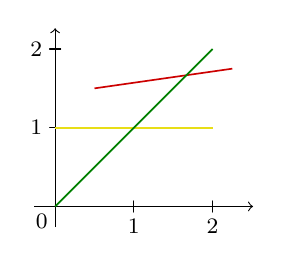
\begin{tikzpicture}
  \datavisualization data group {lines} = {
    data point [x=0, y=0,       set=normal]
    data point [x=2, y=2,       set=normal]
    data point [x=0, y=1,       set=heated]
    data point [x=2, y=1,       set=heated]
    data point [x=0.5, y=1.5,   set=critical]
    data point [x=2.25, y=1.75, set=critical]
  };
  \datavisualization [
    school book axes,
    visualize as line=normal,
    visualize as line=heated,
    visualize as line=critical,
    /data point/set/normal/.initial=1,
    /data point/set/heated/.initial=2,
    /data point/set/critical/.initial=3,
    style sheet=traffic light]
  data group {lines};
\end{tikzpicture}
\end{codeexample}

Now, it is a bit bothersome that we have to set all these |/data point/set/...|
keys by hand. It turns out that this is not necessary: Each time a visualizer
is created, a subkey of |/data point/set| with the name of the visualizer is
created automatically and a number is stored that is increased for each new
visualizer in a data visualization. This means that the three lines starting
with |/data point| are inserted automatically for you, so they can be left out.
However, you would need them for instance when you would like several different
data sets to use the same styling:
%
\begin{codeexample}[]
% Definition of traffic light keys as above
\tikz \datavisualization [
  school book axes,
  visualize as line=normal,
  visualize as line=heated,
  visualize as line=critical,
  /data point/set/critical/.initial=1, % same styling as first set
  style sheet=traffic light]
data group {lines};
\end{codeexample}

We can a command that slightly simplifies the definition of style sheets:

\begin{command}{\pgfdvdeclarestylesheet\marg{name}\marg{keys}}
    This command executes the \meta{keys} with the path prefix
    |/pgf/data visualization/style sheets/|\penalty0\meta{name}. The above
    definition of the traffic light style sheet could be rewritten as follows:
    %
\begin{codeexample}[code only]
\pgfdvdeclarestylesheet{traffic light}{
  1/.style={green!50!black},
  2/.style={yellow!90!black},
  3/.style={red!80!black},
  default style/.style={black}
}
\end{codeexample}
    %
\end{command}

As a final example, let us create a style sheet that changes the dashing
pattern according to the value of the attribute. We do not need to define an
large number of styles in this case, but can use the |default style| key to
``calculate'' the correct dashing.

\begin{codeexample}[]
\pgfdvdeclarestylesheet{my dashings}{
  default style/.style={dash pattern={on #1pt off 1pt}}
}
\tikz \datavisualization [
  school book axes,
  visualize as line=normal,
  visualize as line=heated,
  visualize as line=critical,
  style sheet=my dashings]
data group {lines};
\end{codeexample}


\subsubsection{Creating a New Color Style Sheet}

Creating a style sheet that varies colors according to an attribute works the
same way as creating a normal style sheet: Subkeys lies |1|, |2|, and so on use
the |style| attribute to setup a color. However, instead of using the |color|
attribute to set the color, you should use the |visualizer color| key to set
the color:

\begin{key}{/tikz/visualizer color=\meta{color}}
    This key is used to set the color |visualizer color| to \meta{color}. This
    color is used by visualizers to color the data they visualize, rather than
    the current ``standard color''. The reason for not using the normal current
    color is simply that it makes many internals of the data visualization
    engine a bit simpler.
    %
\begin{codeexample}[]
\pgfdvdeclarestylesheet{my colors}
{
  default style/.style={visualizer color=black},
  1/.style={visualizer color=black},
  2/.style={visualizer color=red!80!black},
  3/.style={visualizer color=blue!80!black},
}
\tikz \datavisualization [
  school book axes,
  visualize as line=normal,
  visualize as line=heated,
  visualize as line=critical,
  style sheet=my colors]
data group {lines};
\end{codeexample}
    %
\end{key}

There is an additional command that makes it easy to define a style sheet based
on a \emph{color series}. Color series are a concept from the |xcolor| package:
The idea is that we start with a certain color for the first data set and then
add a certain ``color offset'' for each next data point. Please consult the
documentation of the |xcolor| package for details.

\begin{command}{\tikzdvdeclarestylesheetcolorseries\marg{name}\marg{color model}\marg{initial color}\marg{step}}
    This command creates a new style sheet using |\pgfdvdeclarestylesheet|.
    This style sheet will only have a default style setup that maps numbers to
    the color in the color series starting with \meta{initial color} and having
    a stepping of \meta{step}. Note that when the value of the attribute is
    |1|, which it is the first data set, the \emph{second} color in the color
    series is used (since counting starts at |0| for color series). Thus, in
    general, you need to start the \meta{initial color} ``one early''.
    %
\begin{codeexample}[]
\tikzdvdeclarestylesheetcolorseries{greens}{hsb}{0.3,1.3,0.8}{0,-.4,-.1}
\tikz \datavisualization [
  school book axes,
  visualize as line=normal,
  visualize as line=heated,
  visualize as line=critical,
  style sheet=greens]
data group {lines};
\end{codeexample}
    %
\end{command}


\subsection{Reference: Style Sheets for Lines}

The following style sheets can be applied to visualizations that use the
|visualize as line| and related keys. For the examples, the following style and
data set are used:
%
\begin{codeexample}[code only]
\tikzdatavisualizationset {
  example visualization/.style={
    scientific axes=clean,
    y axis={ticks={style={
          /pgf/number format/fixed,
          /pgf/number format/fixed zerofill,
          /pgf/number format/precision=2}}},
    x axis={ticks={tick suffix=${}^\circ$}},
    1={label in legend={text=$\frac{1}{6}\sin 11x$}},
    2={label in legend={text=$\frac{1}{7}\sin 12x$}},
    3={label in legend={text=$\frac{1}{8}\sin 13x$}},
    4={label in legend={text=$\frac{1}{9}\sin 14x$}},
    5={label in legend={text=$\frac{1}{10}\sin 15x$}},
    6={label in legend={text=$\frac{1}{11}\sin 16x$}},
    7={label in legend={text=$\frac{1}{12}\sin 17x$}},
    8={label in legend={text=$\frac{1}{13}\sin 18x$}}
  }
}
\end{codeexample}
\tikzdatavisualizationset {
  example visualization/.style={
    scientific axes=clean,
    y axis={ticks={style={
          /pgf/number format/fixed,
          /pgf/number format/fixed zerofill,
          /pgf/number format/precision=2}}},
    x axis={ticks={tick suffix=${}^\circ$}},
    1={label in legend={text=$\frac{1}{6}\sin 11x$}},
    2={label in legend={text=$\frac{1}{7}\sin 12x$}},
    3={label in legend={text=$\frac{1}{8}\sin 13x$}},
    4={label in legend={text=$\frac{1}{9}\sin 14x$}},
    5={label in legend={text=$\frac{1}{10}\sin 15x$}},
    6={label in legend={text=$\frac{1}{11}\sin 16x$}},
    7={label in legend={text=$\frac{1}{12}\sin 17x$}},
    8={label in legend={text=$\frac{1}{13}\sin 18x$}}
  }
}

\begin{codeexample}[code only]
\tikz \datavisualization data group {sin functions} = {
  data [format=function] {
    var set : {1,...,8};
    var x : interval [0:50];
    func y = sin(\value x * (\value{set}+10))/(\value{set}+5);
  }
};
\end{codeexample}
\tikz \datavisualization data group {sin functions} = {
  data [format=function] {
    var set : {1,...,8};
    var x : interval [0:50];
    func y = sin(\value x * (\value{set}+10))/(\value{set}+5);
  }
};

\begin{stylesheet}{vary thickness}
    This style varies the thickness of lines. It should be used only when there
    are only two or three lines, and even then it is not particularly pleasing
    visually.
    %
\begin{codeexample}[width=10cm]
\tikz \datavisualization [
  visualize as smooth line/.list=
    {1,2,3,4,5,6,7,8},
  example visualization,
  style sheet=vary thickness]
data group {sin functions};
\end{codeexample}
    %
\end{stylesheet}

\begin{stylesheet}{vary dashing}
    This style varies the dashing of lines. Although it is not particularly
    pleasing visually and although visualizations using this style sheet tend
    to look ``excited'' (but not necessarily ``exciting''), this style sheet is
    often the best choice when the visualization is to be printed in black and
    white.
    %
\begin{codeexample}[width=10cm]
\tikz \datavisualization [
  visualize as smooth line/.list=
    {1,2,3,4,5,6,7,8},
  example visualization,
  style sheet=vary dashing]
data group {sin functions};
\end{codeexample}
    %
    As can be seen, there are only seven distinct dashing patterns. The eighth
    and further lines will use a solid line once more. You will then have to
    specify the dashing ``by hand'' using the |style| option together with the
    visualizer.
\end{stylesheet}

\begin{stylesheet}{vary dashing and thickness}
    This style alternates between varying the thickness and the dashing of
    lines. The difference to just using both the |vary thickness| and
    |vary dashing| is that too thick lines are avoided. Instead, this style
    creates clearly distinguishable line styles for many lines (up to 14) with
    a minimum of visual clutter. This style is the most useful for
    visualizations when many different lines (ten or more) should be printed in
    black and white.
    %
\begin{codeexample}[width=10cm]
\tikz \datavisualization [
  visualize as smooth line/.list=
    {1,2,3,4,5,6,7,8},
  example visualization,
  style sheet=vary thickness
              and dashing]
data group {sin functions};
\end{codeexample}
    %
    For comparison, here is the must-less-than-satisfactory result of combining
    the two independent style sheets:
    %
\begin{codeexample}[width=10cm]
\tikz \datavisualization [
  visualize as smooth line/.list=
    {1,2,3,4,5,6,7,8},
  example visualization,
  style sheet=vary thickness,
  style sheet=vary dashing]
data group {sin functions};
\end{codeexample}
    %
\end{stylesheet}


\subsection{Reference: Style Sheets for Scatter Plots}

The following style sheets can be used both for scatter plots and also with
lines. In the latter case, the marks are added to the lines.

\begin{stylesheet}{cross marks}
    This style uses different crosses to distinguish between the data points of
    different data sets. The crosses were chosen in such a way that when two
    different cross marks lie at the same coordinate, their overall shape
    allows one to still uniquely determine which marks are on top of each
    other.

    This style supports only up to six different data sets and requires the
    |plotmarks| library.
    %
\begin{codeexample}[width=10cm]
\tikz \datavisualization [
  visualize as scatter/.list=
    {1,2,3,4,5,6,7,8},
  example visualization,
  style sheet=cross marks]
data group {sin functions};
\end{codeexample}
    %
\begin{codeexample}[width=10cm]
\tikz \datavisualization [
  visualize as smooth line/.list=
    {1,2,3,4,5,6,7,8},
  example visualization,
  style sheet=cross marks]
data group {sin functions};
\end{codeexample}
    %
\end{stylesheet}


\subsection{Reference: Color Style Sheets}

Color style sheets are very useful for creating visually pleasing data
visualizations that contain multiple data sets. However, there are two things
to keep in mind:
%
\begin{itemize}
    \item At some point, every data visualization is printed or photo copied in
        black and white by someone. In this case, data sets can often no longer
        be distinguished.
    \item A few people are color blind. They will not be able to distinguish
        between red and green lines (and some people are not even able to
        distinguish colors at all).
\end{itemize}

For these reasons, if there is any chance that the data visualization will be
printed in black and white at some point, consider combining color style sheets
with style sheets like |vary dashing| to make data sets distinguishable in all
situations.

\begin{stylesheet}{strong colors}
    This style sheets uses pure primary colors that can very easily be
    distinguished. Although not as visually pleasing as the |vary hue| style
    sheet, the visualizations are easier to read when this style sheet is used.
    Up to six different data sets are supported.
    %
\begin{codeexample}[width=10cm]
\tikz \datavisualization [
  visualize as smooth line/.list=
    {1,2,3,4,5,6,7,8},
  example visualization,
  style sheet=strong colors]
data group {sin functions};
\end{codeexample}
    %
\begin{codeexample}[width=10cm]
\tikz \datavisualization [
  visualize as smooth line/.list=
    {1,2,3,4,5,6,7,8},
  example visualization,
  style sheet=strong colors,
  style sheet=vary dashing]
data group {sin functions};
\end{codeexample}
    %
\end{stylesheet}


Unlike |strong colors|, the following style sheets support, in principle, an
unlimited number of data set. In practice, as always, more than four or five
data sets lead to nearly indistinguishable data sets.

\begin{stylesheet}{vary hue}
    This style uses a different hue for each data set.
    %
\begin{codeexample}[width=10cm]
\tikz \datavisualization [
  visualize as smooth line/.list=
    {1,2,3,4,5,6,7,8},
  example visualization,
  style sheet=vary hue]
data group {sin functions};
\end{codeexample}
    %
\end{stylesheet}

\begin{stylesheet}{shades of blue}
    As the name suggests, different shades of blue are used for different data
    sets.
\begin{codeexample}[width=10cm]
\tikz \datavisualization [
  visualize as smooth line/.list=
    {1,2,3,4,5,6,7,8},
  example visualization,
  style sheet=shades of blue]
data group {sin functions};
\end{codeexample}
    %
\end{stylesheet}

\begin{stylesheet}{shades of red}
\begin{codeexample}[width=10cm]
\tikz \datavisualization [
  visualize as smooth line/.list=
    {1,2,3,4,5,6,7,8},
  example visualization,
  style sheet=shades of red]
data group {sin functions};
\end{codeexample}
\end{stylesheet}

\begin{stylesheet}{gray scale}
    For once, this style sheet can also be used when the visualization is
    printed in black and white.
    %
\begin{codeexample}[width=10cm]
\tikz \datavisualization [
  visualize as smooth line/.list=
    {1,2,3,4,5,6,7,8},
  example visualization,
  style sheet=gray scale]
data group {sin functions};
\end{codeexample}
    %
\end{stylesheet}


\subsection{Usage: Labeling Data Sets Inside the Visualization}

In a visualization that contains multiple data sets, it is often necessary to
clearly point out which line or mark type corresponds to which data set. This
can be done in the main text via a sentence like ``the normal data (black) lies
clearly below the critical values (red)'', but it often a good idea to indicate
data sets ideally directly inside the data visualization or directly next to it
in a so-called legend.

The data visualization engine has direct support both for indicating data sets
directly inside the visualization and also for indicating them in a legend.

The ``best'' way of indicating where a data set lies or which color is used for
it is to put a label directly inside the data visualization. The reason this is
the ``best'' way is that people do not have to match the legend entries against
the data, let alone having to look up the meaning of line styles somewhere in
the text. However, adding a label directly inside the visualization is also the
most tricky way of indicating data sets since it is hard to compute good
positions for the labels automatically and since there needs to be some empty
space where the label can be put.


\subsubsection{Placing a Label Next to a Data Set}

The following key is used to create a label inside the data visualization for a
data set:

\begin{key}{/tikz/data visualization/visualizer options/label in data=\meta{options}}
    This key is passed to a visualizer that has previously been created using
    keys starting |visualize as ...|. It will create a label inside the data
    visualization ``next'' to the visualizer (the details are explained in a
    moment). You can use this key multiple times with a visualizer to create
    multiple labels at different points with different texts.

    The \meta{options} determine which text is shown and where it is shown.
    They are executed with the following path prefix:
    %
\begin{codeexample}[code only]
/tikz/data visualization/visualizer label options
\end{codeexample}

    In order to configure which text is shown and where, use the following keys
    inside the \meta{options}:

    \begin{key}{/tikz/data visualization/visualizer label options/text=\meta{text}}
        This is the text that will be displayed next to the data. It will be to
        the ``left'' of the data, see the description below.
    \end{key}
    %
    \begin{key}{/tikz/data visualization/visualizer label options/text'=\meta{text}}
        Like |text|, only the text will be to the ``right'' of the data.
    \end{key}

    The following keys are used to configure where the label will be shown.
    They use different strategies to specify one data point where the label
    will be anchored. The coordinate of this data point will be stored in
    |(label| |visualizer| |coordinate)|. Independently of the strategy, once
    the data point has been chosen, the coordinate of the next data point is
    stored in |(label| |visualizer| |coordinate')|. Then, a (conceptual) line
    is created from the first coordinate to the second and a node is placed at
    the beginning of this line to its ``left'' or, for the |text'| option, on
    its ``right''. More precisely, an automatic anchor is computed for a node
    placed implicitly on this line using the |auto| option or, for the |text'|
    option, using |auto,swap|.

    The node placed at the position computed in this way will have the
    \meta{text} set by the |text| or |text'| option and its styling is
    determined by the current |node style|.

    Let us now have a look at the different ways of determining the data point
    at which the label in anchored:
    %
    \begin{key}{/tikz/data visualization/visualizer label options/when=\meta{attribute}| is|\meta{number}}
        This key causes the value of the \meta{attribute} to be monitored in
        the stream of data points. The chosen is data point is the first data
        point where the \meta{attribute} is at least \meta{number} (if this
        never happens, the last data point is used).
        %
\begin{codeexample}[width=6.3cm]
\tikz \datavisualization [
  school book axes,
  x axis={label=$x$},
  visualize as smooth line/.list={log, lin, squared, exp},
  log=    {label in data={text'=$\log x$, when=y is -1,
                          text colored}},
  lin=    {label in data={text=$x/2$,     when=x is 2}},
  squared={label in data={text=$x^2$,     when=x is 1.1}},
  exp=    {label in data={text=$e^x$,     when=x is -2,
                          text colored}},
  style sheet=vary hue]
data group {function classes};
\end{codeexample}
    \end{key}
    %
    \begin{key}{/tikz/data visualization/visualizer label options/index=\meta{number}}
        This key chooses the \meta{number}th data point belonging to the
        visualizer's data set.
        %
\begin{codeexample}[width=6.3cm]
\tikz \datavisualization [
  school book axes,
  x axis={label=$x$},
  visualize as smooth line/.list={exp},
  exp=    {label in data={text=$5$, index=5},
           label in data={text=$10$, index=10},
           label in data={text=$20$, index=20},
           style={mark=x}},
  style sheet=vary hue]
data group {function classes};
\end{codeexample}
    \end{key}
    %
    \begin{key}{/tikz/data visualization/visualizer label options/pos=\meta{fraction}}
        This key chooses the first data point belonging to the data set whose
        index is at least \meta{fraction} times the number of all data points
        in the data set.
        %
\begin{codeexample}[width=6.3cm]
\tikz \datavisualization [
  school book axes,
  x axis={label=$x$},
  visualize as smooth line=exp,
  exp=    {label in data={text=$.2$, pos=0.2},
           label in data={text=$.5$, pos=0.5},
           label in data={text=$.95$, pos=0.95},
           style={mark=x}},
  style sheet=vary hue]
data group {function classes};
\end{codeexample}
    \end{key}
    %
    \begin{key}{/tikz/data visualization/visualizer label options/auto}
        This key is executed automatically by default. It works like the |pos|
        option, where the \meta{fraction} is set to $(\meta{data set's
        index}-1/2)/\meta{number of data sets}$. For instance, when there are
        $10$ data sets, the fraction for the first one will be $5\%$, the
        fraction for the second will be $15\%$, for the third it will be
        $25\%$, ending with $95\%$ for the last one.

        The net effect of all this is that when there are several lines, labels
        will be placed at different positions along the lines with hopefully
        only little overlap.
        %
\begin{codeexample}[width=6.3cm]
\tikz \datavisualization [
  scientific axes=clean,
  visualize as smooth line/.list={linear, squared, cubed},
  linear ={label in data={text=$2x$}},
  squared={label in data={text=$x^2$}},
  cubed  ={label in data={text=$x^3$}}]
data [set=linear, format=function] {
  var x : interval [0:1.5];
  func y = 2*\value x;
}
data [set=squared, format=function] {
  var x : interval [0:1.5];
  func y = \value x * \value x;
}
data [set=cubed, format=function] {
  var x : interval [0:1.5];
  func y = \value x * \value x * \value x;
};
\end{codeexample}
        %
        As can be seen in the example, the result is not always satisfactory.
        In this case, the |pin in data| option might be preferable, see below.
    \end{key}

    The following keys allow you to style labels.

    \begin{key}{/tikz/data visualization/visualizer label options/node style=\meta{options}}
        Just passes the options to |/tikz/data visualization/node style|.
    \end{key}
    %
    \begin{key}{/tikz/data visualization/visualizer label options/text colored}
        Causes the |node style| to set the text color to |visualizer color|.
        The effect of this is that the label's text will have the same color as
        the data set to which it is attached.
    \end{key}

    \begin{stylekey}{/tikz/data visualization/every data set label}
        This style is executed with every label that represents a data set.
        Inside this style, use |node style| to change the appearance of nodes.
        This style has a default definition, usually you should just append
        things to this style.
        %
\begin{codeexample}[width=6.3cm]
\tikz \datavisualization [
  school book axes,
  x axis={label=$x$},
  visualize as smooth line/.list={log, lin, squared, exp},
  every data set label/.append style={text colored},
  log=    {label in data={text'=$\log x$, when=y is -1}},
  lin=    {label in data={text=$x/2$,
                    node style=sloped,    when=x is 2}},
  squared={label in data={text=$x^2$,     when=x is 1.1}},
  exp=    {label in data={text=$e^x$,
                    node style=sloped,    when=x is -2}},
  style sheet=vary hue]
data group {function classes};
\end{codeexample}
    \end{stylekey}

    \begin{stylekey}{/tikz/data visualization/every label in data}
        Like |every data set label|, this key is also executed with labels.
        However, this key is executed after the style sheets have been
        executed, giving you a chance to overrule their styling.
    \end{stylekey}
\end{key}


\subsubsection{Connecting a Label to a Data Set via a Pin}

\begin{key}{/tikz/data visualization/visualizer options/pin in data=\meta{options}}
    This key is a variant of the |label in data| key and takes the same
    options, plus two additional ones. The difference to |label in data| is
    that the label node is shown a bit removed from the data set, but connected
    to it via a small line (this is like the difference between the |label| and
    |pin| options).
    %
\begin{codeexample}[width=6.3cm]
\tikz \datavisualization [
  scientific axes=clean,
  visualize as smooth line/.list={linear, squared, cubed},
  linear ={pin in data={text=$2x$}},
  squared={pin in data={text=$x^2$}},
  cubed  ={pin in data={text=$x^3$}}]
data [set=linear, format=function] {
  var x : interval [0:1.5];
  func y = \value x;
}
data [set=squared, format=function] {
  var x : interval [0:1.5];
  func y = \value x * \value x;
}
data [set=cubed, format=function] {
  var x : interval [0:1.5];
  func y = \value x * \value x * \value x;
};
\end{codeexample}
    %
    The following keys can be used additionally:
    %
    \begin{key}{/tikz/data visualization/visualizer label options/pin angle=\meta{angle}}
        The position of the label of a |pin in data| is mainly computed in the
        same way as for a |label in data|. However, once the position has been
        computed, the label is shifted as follows:
        %
        \begin{itemize}
            \item When an \meta{angle} is specified using the present key, the
                shift is by the current value of |pin length| in the direction
                of \meta{angle}.
            \item When \meta{angle} is empty (which is the default), then the
                shift is also by the current value of |pin length|, but now in
                the direction that is orthogonal and to the left of the line
                between the coordinate of the data point and the coordinate of
                the next data point. When |text'| is used, the direction is to
                the right instead of the left.
        \end{itemize}
    \end{key}

    \begin{key}{/tikz/data visualization/visualizer label options/pin length=\meta{dimension}}
        See the description of |pin angle|.
    \end{key}
    %
\begin{codeexample}[width=6.3cm]
\tikz \datavisualization [
  school book axes,
  x axis={label=$x$},
  visualize as smooth line/.list={log, lin, squared, exp},
  every data set label/.append style={text colored},
  log=    {pin in data={text'=$\log x$, when=y is -1}},
  lin=    {pin in data={text=$x/2$, when=x is 2,
                        pin length=1ex}},
  squared={pin in data={text=$x^2$, when=x is 1.1,
                        pin angle=230}},
  exp=    {label in data={text=$e^x$, when=x is -2}},
  style sheet=vary hue]
data group {function classes};
\end{codeexample}
    \end{key}


\subsection{Usage: Labeling Data Sets Inside a Legend}

The ``classical'' way of indicating the style used for the different data sets
inside a visualization is a \emph{legend}. It is a description next to or even
inside the visualization that contains one line for each data set and displays
an iconographic version of the data set next to some text labeling the data
set. Note, however, that even though legend are quite common, also consider
using a |label in data| or a |pin in data| instead.

Creating a high-quality legend is by no means simple. A legend should not
distract the reader, so aggressive borders should definitively be avoided. A
legend should make it easy to match the actual styling of a data set (like,
say, using a red, dashed line) to the ``iconographic'' representation of this
styling. An example of what can go wrong here is using short lines to represent
lines dashed in different way where the lines are so short that the differences
in the dashing cannot be discerned. Another example is showing straight lines
with plot marks on them where the plot marks are obscured by the horizontal
line itself, while the plot marks are clearly visible in the actual
visualization since no horizontal lines occur.

The data visualization engine comes with a large set of options for creating
and placing high-quality legends next or inside data visualizations.


\subsubsection{Creating Legends and Legend Entries}

A data visualization can be accompanied by one or more legends. In order to
create a legend, the following key can be used (although, in practice, you will
usually use the |legend| key instead, see below):

\begin{key}{/tikz/data visualization/new legend=\meta{legend name} (default main legend)}
    This key is used to create a new legend named \meta{legend name}. The
    legend is empty by default and further options are needed to add entries to
    it. When the key is called a second time for the same \meta{legend name}
    nothing happens.

    When a legend is created, a new key is created that can subsequently be
    used to configure the legend:
    %
    \begin{key}{/tikz/data visualization/\meta{legend name}=\meta{options}}
        When this key is used, the \meta{options} are executed with the path
        prefix
        %
\begin{codeexample}[code only]
/tikz/data visualization/legend options
\end{codeexample}
        %
        The different keys with this path prefix allow you to change the
        position where the legend is shown and how it is organised (for
        instance, whether legend entries are shown in a row or in a column or
        in a square).

        The different possible keys will be explained in the course of this
        section.
    \end{key}

    In the end, the legend is just a \tikzname\ node, a |matrix| node, to be
    precise. The following key is used to style this node:

    \begin{key}{/tikz/data visualization/legend options/matrix node style=\meta{options}}
        Adds the \meta{options} to the list of options that will be executed
        when the legend's node is created.
        %
\begin{codeexample}[width=8cm]
\tikz \datavisualization [
  scientific axes,
  visualize as smooth line/.list=
    {log, lin, squared, exp},
  legend={matrix node style={fill=black!25}},
  log=    {label in legend={text=$\log x$}},
  lin=    {label in legend={text=$x/2$}},
  squared={label in legend={text=$x^2$}},
  exp=    {label in legend={text=$e^x$}},
  style sheet=vary dashing]
data group {function classes};
\end{codeexample}
    \end{key}

    The following style allows you to configure the default appearance of every
    newly created legend:
    %
    \begin{stylekey}{/tikz/data visualization/legend options/every new legend}
        This key defaults to |east outside, label style=text right|. This means
        that by default a legend is placed to the right of the data
        visualization and that in the individual legend entries the text is to
        the right of the data set visualization.
    \end{stylekey}
    %
\begin{codeexample}[width=6cm]
\tikz \datavisualization [
  scientific axes, x axis={label=$x$},
  visualize as smooth line/.list={log, lin, squared, exp},
  new legend={upper legend},
  new legend={lower legend},
  upper legend=above,
  lower legend=below,
  log=    {label in legend={text=$\log x$, legend=upper legend}},
  lin=    {label in legend={text=$x/2$, legend=upper legend}},
  squared={label in legend={text=$x^2$, legend=lower legend}},
  exp=    {label in legend={text=$e^x$, legend=lower legend}},
  style sheet=vary dashing]
data group {function classes};
\end{codeexample}
    %
\end{key}

\begin{key}{/tikz/data visualization/legend=\meta{options}}
    This is a shorthand for
    |new legend=main legend, main legend=|\meta{options}. In other words, this
    key creates a new |main legend| and immediately passes the configuration
    \meta{options} to this legend.
    %
\begin{codeexample}[width=7cm]
\tikz \datavisualization [
  scientific axes, x axis={label=$x$},
  visualize as smooth line/.list={log, lin, squared, exp},
  legend=below,
  log=    {label in legend={text=$\log x$}},
  lin=    {label in legend={text=$x/2$}},
  squared={label in legend={text=$x^2$}},
  exp=    {label in legend={text=$e^x$}},
  style sheet=vary dashing]
data group {function classes};
\end{codeexample}
    %
\end{key}

As pointed out above, a legend is empty by default. In particular, the
different data sets are not automatically inserted into the legend. Instead,
the key |label in legend| must be used together with a data set:

\begin{key}{/tikz/data visualization/visualizer options/label in legend=\meta{options}}
    This key is passed to a data set, similar to options like |pin in data| or
    |smooth line|. The \meta{options} are used to configure the following:
    %
    \begin{itemize}
        \item The legend in which the data set should be visualized.
        \item The text that is to be shown in the legend for the data set.
        \item The appearance of the legend entries.
    \end{itemize}
    %
    In detail, the \meta{options} are executed with the path prefix
    %
\begin{codeexample}[code only]
/tikz/data visualization/legend entry options
\end{codeexample}
    %
    To configure in which legend the label should appear, use the
    following key:
    %
    \begin{key}{/tikz/data visualization/legend entry options/legend=\meta{name} (initially main legend)}
        Set this key to the name of a legend that has previously been created
        using |new legend|. The label will then be shown in this legend.

        In most cases, there is only one legend (namely |main legend|) and
        there is no need to set this key since it defaults to the main legend.

        Also note that the legend \meta{name} is automatically created if it
        nodes not yet exist.
    \end{key}

    \begin{key}{/tikz/data visualization/legend entry options/text=\meta{text}}
        Use this key to setup the \meta{text} that is shown as the label of the
        data set.
        %
\begin{codeexample}[width=8cm]
\tikz \datavisualization [
  scientific axes, x axis={label=$x$},
  visualize as smooth line/.list=
  {log, lin, squared, exp},
  log=    {label in legend={text=$\log x$}},
  lin=    {label in legend={text=$x/2$}},
  squared={pin in data    ={text=$x^2$, pos=0.1}},
  exp=    {label in data  ={text=$e^x$}},
  style sheet=vary dashing]
data group {function classes};
\end{codeexample}
    \end{key}

    In addition to the two keys described above, there are further keys that
    are described in Section~\ref{section-dv-label-legend-entry-options}.
\end{key}


\subsubsection{Rows and Columns of Legend Entries}

In a legend, the different legend entries are arranged in a matrix, which
typically has only one row or one column. For the impatient reader: Say
|rows=1| to get everything in a row, say |columns=1| to get everything in a
single column, and skip the rest of this section.

The more patient reader will appreciate that when there are very many different
data sets in a single visualization, it may be necessary to use more than one
row or column inside the legend. \tikzname\ comes with a rather powerful
mechanism for distributing the multiple legend entries over the matrix.

The first thing to decide is in which ``direction'' the entries should be
inserted into the matrix. Suppose we have a $3 \times 3$ matrix and our entries
are $a$, $b$, $c$, and so on. Then, one might place the $a$ in the upper left
corner of the matrix, $b$ in the upper middle position, $c$ in the upper right
position, and $d$ in the middle left position. This is a ``first right, then
down'' strategy. A different strategy might be to place the $a$ in the upper
left corner, but $b$ in the middle left position, $c$ in the lower left
position, and $d$ then in the upper middle position. This is a ``first down,
then right'' strategy. In certain situations it might even make sense to place
$a$ in the lower right corner and then go ``first up, then left''.

All of these strategies are supported by the |legend| command. You can
configure which strategy is used using the following keys:

\tikzdatavisualizationset {
  legend example/.style={
    scientific axes, all axes={length=1cm, ticks=none},
    1={label in legend={text=1}},
    2={label in legend={text=2}},
    3={label in legend={text=3}},
    4={label in legend={text=4}},
    5={label in legend={text=5}},
    6={label in legend={text=6}},
    7={label in legend={text=7}},
    8={label in legend={text=8}}
  }
}

\begin{key}{/tikz/data visualization/legend options/down then right}
    Causes the legend entries to fill the legend matrix first downward and,
    once a column is full, the next column is begun to the right of the
    previous one. This is the default.
    %
\begin{codeexample}[width=6cm]
\tikz \datavisualization [
  visualize as smooth line/.list={1,2,3,4,5,6,7,8},
  legend example, style sheet=vary hue,
  main legend={down then right, columns=3}]
data group {sin functions};
\end{codeexample}
    %
    In the example, the |legend example| is the following style:
    %
\begin{codeexample}[code only]
\tikzdatavisualizationset {
  legend example/.style={
    scientific axes, all axes={length=1cm, ticks=none},
    1={label in legend={text=1}},
    2={label in legend={text=2}},
    3={label in legend={text=3}},
    4={label in legend={text=4}},
    5={label in legend={text=5}},
    6={label in legend={text=6}},
    7={label in legend={text=7}},
    8={label in legend={text=8}}
  }
}
\end{codeexample}
    %
\end{key}

\begin{key}{/tikz/data visualization/legend options/down then left}
\begin{codeexample}[width=6cm]
\tikz \datavisualization [
  visualize as smooth line/.list={1,2,3,4,5,6,7,8},
  legend example, style sheet=vary hue,
  main legend={down then left, columns=3}]
data group {sin functions};
\end{codeexample}
\end{key}

\begin{key}{/tikz/data visualization/legend options/up then right}
\begin{codeexample}[width=6cm]
\tikz \datavisualization [
  visualize as smooth line/.list={1,2,3,4,5,6,7,8},
  legend example, style sheet=vary hue,
  main legend={up then right, columns=3}]
data group {sin functions};
\end{codeexample}
\end{key}

\begin{key}{/tikz/data visualization/legend options/up then left}
\begin{codeexample}[width=6cm]
\tikz \datavisualization [
  visualize as smooth line/.list={1,2,3,4,5,6,7,8},
  legend example, style sheet=vary hue,
  main legend={up then left, columns=3}]
data group {sin functions};
\end{codeexample}
\end{key}

\begin{key}{/tikz/data visualization/legend options/left then up}
\begin{codeexample}[width=6cm]
\tikz \datavisualization [
  visualize as smooth line/.list={1,2,3,4,5,6,7,8},
  legend example, style sheet=vary hue,
  main legend={left then up, columns=3}]
data group {sin functions};
\end{codeexample}
\end{key}

\begin{key}{/tikz/data visualization/legend options/left then down}
\begin{codeexample}[width=6cm]
\tikz \datavisualization [
  visualize as smooth line/.list={1,2,3,4,5,6,7,8},
  legend example, style sheet=vary hue,
  main legend={left then down, columns=3}]
data group {sin functions};
\end{codeexample}
\end{key}

\begin{key}{/tikz/data visualization/legend options/right then up}
\begin{codeexample}[width=6cm]
\tikz \datavisualization [
  visualize as smooth line/.list={1,2,3,4,5,6,7,8},
  legend example, style sheet=vary hue,
  main legend={right then up, columns=3}]
data group {sin functions};
\end{codeexample}
\end{key}

\begin{key}{/tikz/data visualization/legend options/right then down}
\begin{codeexample}[width=6cm]
\tikz \datavisualization [
  visualize as smooth line/.list={1,2,3,4,5,6,7,8},
  legend example, style sheet=vary hue,
  main legend={right then down, columns=3}]
data group {sin functions};
\end{codeexample}
\end{key}

Having configured the directions in which the matrix is being filled, you must
next setup the number of rows or columns that are to be shown. There are
actually two different ways of doing so. The first way is to specify a maximum
number of rows or columns. For instance, you might specify that there should be
at most ten rows to a column and when there are more, a new column should be
begun. This is achieved using the following keys:

\begin{key}{/tikz/data visualization/legend options/max rows=\meta{number}}
    As the legend matrix is being filled, whenever the number of rows in the
    current column would exceed \meta{number}, a new column is started.
    %
\begin{codeexample}[width=7cm]
\tikz \datavisualization [
  visualize as smooth line/.list={1,2,3,4,5,6,7,8},
  legend example, style sheet=vary hue,
  main legend={max rows=3}]
data group {sin functions};
\end{codeexample}
    %
\begin{codeexample}[width=7cm]
\tikz \datavisualization [
  visualize as smooth line/.list={1,2,3,4,5,6,7,8},
  legend example, style sheet=vary hue,
  main legend={max rows=4}]
data group {sin functions};
\end{codeexample}
    %
\begin{codeexample}[width=7cm]
\tikz \datavisualization [
  visualize as smooth line/.list={1,2,3,4,5,6,7,8},
  legend example, style sheet=vary hue,
  main legend={max rows=5}]
data group {sin functions};
\end{codeexample}
    %
\end{key}

\begin{key}{/tikz/data visualization/legend options/max columns=\meta{number}}
    This key works like |max rows|, only now the number of columns is
    monitored. Note that this strategy only really makes sense when the when
    you use this key with a strategy that first goes left or right and then up
    or down.
    %
\begin{codeexample}[width=7cm]
\tikz \datavisualization [
  visualize as smooth line/.list={1,2,3,4,5,6,7,8},
  legend example, style sheet=vary hue,
  main legend={right then down, max columns=2}]
data group {sin functions};
\end{codeexample}
    %
\begin{codeexample}[width=7cm]
\tikz \datavisualization [
  visualize as smooth line/.list={1,2,3,4,5,6,7,8},
  legend example, style sheet=vary hue,
  main legend={right then down,max columns=3}]
data group {sin functions};
\end{codeexample}
    %
\begin{codeexample}[width=7cm]
\tikz \datavisualization [
  visualize as smooth line/.list={1,2,3,4,5,6,7,8},
  legend example, style sheet=vary hue,
  main legend={right then down,max columns=4}]
data group {sin functions};
\end{codeexample}
    %
\end{key}

The second way of specifying the number of entries in a row or column is to
specify an ``ideal number of rows or columns''. The idea is as follows: Suppose
that we use the standard strategy and would like to have everything in two
columns. Then if there are eight entries, the first four should go to the first
column, while the next four should go to the second column. If we have 20
entries, the first ten should go the first column and the next ten to the
second, and so on. So, in general, the objective is to distribute the entries
evenly so the this ``ideal number of columns'' is reached. Only when there are
too few entries to achieve this or when the number of entries per column would
exceed the |max rows| value, will the number of columns deviate from this ideal
value.

\begin{key}{/tikz/data visualization/legend options/ideal number of columns=\meta{number}}
    Specifies, that the entries should be split into \meta{number} different
    columns, whenever possible. However, when there would be more than the
    |max rows| value of rows per column, more columns than the ideal number are
    created.
    %
\begin{codeexample}[width=7cm]
\tikz \datavisualization [
  visualize as smooth line/.list={1,2,3,4,5,6,7,8},
  legend example, style sheet=vary hue,
  main legend={ideal number of columns=2}]
data group {sin functions};
\end{codeexample}
    %
\begin{codeexample}[width=7cm]
\tikz \datavisualization [
  visualize as smooth line/.list={1,2,3,4,5,6,7,8},
  legend example, style sheet=vary hue,
  main legend={ideal number of columns=4}]
data group {sin functions};
\end{codeexample}
    %
\begin{codeexample}[width=7cm]
\tikz \datavisualization [
  visualize as smooth line/.list={1,2,3,4,5,6,7,8},
  legend example, style sheet=vary hue,
  main legend={max rows=3,ideal number of columns=2}]
data group {sin functions};
\end{codeexample}
    %
\end{key}

\begin{key}{/tikz/data visualization/legend options/rows=\meta{number}}
    Shorthand for |ideal number of rows=|\meta{number}.
\end{key}

\begin{key}{/tikz/data visualization/legend options/ideal number of rows=\meta{number}}
    Works like |ideal number of columns|.
    %
\begin{codeexample}[width=7cm]
\tikz \datavisualization [
  visualize as smooth line/.list={1,2,3,4,5,6,7,8},
  legend example, style sheet=vary hue,
  main legend={ideal number of rows=2}]
data group {sin functions};
\end{codeexample}
    %
\begin{codeexample}[width=7cm]
\tikz \datavisualization [
  visualize as smooth line/.list={1,2,3,4,5,6,7,8},
  legend example, style sheet=vary hue,
  main legend={ideal number of rows=4}]
data group {sin functions};
\end{codeexample}
    %
\begin{codeexample}[width=7cm]
\tikz \datavisualization [
  visualize as smooth line/.list={1,2,3,4,5,6,7,8},
  legend example, style sheet=vary hue,
  main legend={max columns=3,ideal number of rows=2}]
data group {sin functions};
\end{codeexample}
    %
\end{key}

\begin{key}{/tikz/data visualization/legend options/columns=\meta{number}}
    Shorthand for |ideal number of columns=|\meta{number}.
\end{key}


\subsubsection{Legend Placement: The General Mechanism}

A legend can either be placed next to the data visualization or inside the data
visualization at some place where there are no data entries. Both approached
have advantages: Placing the legend next to the visualization minimises the
``cluttering'' by keeping all the extra information apart from the actual data,
while placing the legend inside the visualization minimises the distance
between the data sets and their explanations, making it easier for the eye to
connect them.

For both approaches there are options that make the placement easier, see
Sections \ref{section-dv-legend-outside} and~\ref{section-dv-legend-inside},
but these options internally just map to the following two options:

\begin{key}{/tikz/data visualization/legend options/anchor=\meta{anchor}}
    The whole legend is a \tikzname-matrix internally. Thus, in particular, it
    is stored in a node, which has anchors. Like for any other node, when the
    node is shown, the node is shifted in such a way that the \meta{anchor} of
    the node lies at the current |at| position.
\end{key}

\begin{key}{/tikz/data visualization/legend options/at=\meta{coordinate}}
    Configures the \meta{coordinate} at which the \meta{anchor} of the legend's
    node should lie.

    It may seem hard to predict a good \meta{coordinate} for a legend since,
    depending of the size of the axis, different positions need to the chosen
    for the legend. However, it turns out that one can often use the
    coordinates of the special nodes |data bounding box| and
    |data visualization bounding box|, documented in
    Section~\ref{section-dv-bounding-box}.

    As an example, let us put a legend to the right of the visualization, but
    so that the first entry starts at the top of the visualization:
    %
\begin{codeexample}[width=8cm]
\tikz \datavisualization [
  scientific axes, x axis={label=$x$},
  visualize as smooth line/.list=
    {log, lin, squared, exp},
  legend={anchor=north west, at=
    (data visualization bounding box.north east)},
  log=    {label in legend={text=$\log x$}},
  lin=    {label in legend={text=$x/2$}},
  squared={label in legend={text=$x^2$}},
  exp=    {label in legend={text=$e^x$}},
  style sheet=vary dashing]
data group {function classes};
\end{codeexample}
    %
    As can be seen, a bit of an additional shift might have been in order, but
    the result is otherwise quite satisfactory.
\end{key}


\subsubsection{Legend Placement: Outside to the Data Visualization}
\label{section-dv-legend-outside}

The following keys make it easy to place a legend outside the data
visualization.

\begin{key}{/tikz/data visualization/legend options/east outside}
    Placing the legend to the right of the data visualization is the default:
    %
\begin{codeexample}[width=8cm]
\tikz \datavisualization [
  scientific axes,
  visualize as smooth line/.list=
    {log, lin, squared, exp},
  legend=east outside,
  log=    {label in legend={text=$\log x$}},
  lin=    {label in legend={text=$x/2$}},
  squared={label in legend={text=$x^2$}},
  exp=    {label in legend={text=$e^x$}},
  style sheet=strong colors]
data group {function classes};
\end{codeexample}

    \begin{key}{/tikz/data visualization/legend options/right}
        This is an easier-to-remember alias.
    \end{key}
\end{key}

\begin{key}{/tikz/data visualization/legend options/north east outside}
    A variant, where the legend is to the right, but aligned with the northern
    end of the data visualization:
    %
\begin{codeexample}[width=8cm]
\tikz \datavisualization [
  scientific axes,
  visualize as smooth line/.list=
    {log, lin, squared, exp},
  legend=north east outside,
  log=    {label in legend={text=$\log x$}},
  lin=    {label in legend={text=$x/2$}},
  squared={label in legend={text=$x^2$}},
  exp=    {label in legend={text=$e^x$}},
  style sheet=strong colors]
data group {function classes};
\end{codeexample}
    %
\end{key}

\begin{key}{/tikz/data visualization/legend options/south east outside}
\begin{codeexample}[width=8cm]
\tikz \datavisualization [
  scientific axes,
  visualize as smooth line/.list=
    {log, lin, squared, exp},
  legend=south east outside,
  log=    {label in legend={text=$\log x$}},
  lin=    {label in legend={text=$x/2$}},
  squared={label in legend={text=$x^2$}},
  exp=    {label in legend={text=$e^x$}},
  style sheet=strong colors]
data group {function classes};
\end{codeexample}
\end{key}

\begin{key}{/tikz/data visualization/legend options/west outside}
    The legend is placed left. Note that the text also swaps its position.
    %
\begin{codeexample}[width=8cm]
\tikz \datavisualization [
  scientific axes,
  visualize as smooth line/.list=
    {log, lin, squared, exp},
  legend=west outside,
  log=    {label in legend={text=$\log x$}},
  lin=    {label in legend={text=$x/2$}},
  squared={label in legend={text=$x^2$}},
  exp=    {label in legend={text=$e^x$}},
  style sheet=strong colors]
data group {function classes};
\end{codeexample}
    %
    \begin{key}{/tikz/data visualization/legend options/left}
        This is an easier-to-remember alias.
    \end{key}
\end{key}

\begin{key}{/tikz/data visualization/legend options/north west outside}
\begin{codeexample}[width=8cm]
\tikz \datavisualization [
  scientific axes,
  visualize as smooth line/.list=
    {log, lin, squared, exp},
  legend=north west outside,
  log=    {label in legend={text=$\log x$}},
  lin=    {label in legend={text=$x/2$}},
  squared={label in legend={text=$x^2$}},
  exp=    {label in legend={text=$e^x$}},
  style sheet=strong colors]
data group {function classes};
\end{codeexample}
\end{key}

\begin{key}{/tikz/data visualization/legend options/south west outside}
\begin{codeexample}[width=8cm]
\tikz \datavisualization [
  scientific axes,
  visualize as smooth line/.list=
    {log, lin, squared, exp},
  legend=south west outside,
  log=    {label in legend={text=$\log x$}},
  lin=    {label in legend={text=$x/2$}},
  squared={label in legend={text=$x^2$}},
  exp=    {label in legend={text=$e^x$}},
  style sheet=strong colors]
data group {function classes};
\end{codeexample}
\end{key}


\begin{key}{/tikz/data visualization/legend options/north outside}
    The legend is placed above the data. Note that the legend entries now for a
    row rather than a column.
    %
\begin{codeexample}[width=8cm]
\tikz \datavisualization [
  scientific axes,
  visualize as smooth line/.list=
    {log, lin, squared, exp},
  legend=north outside,
  log=    {label in legend={text=$\log x$}},
  lin=    {label in legend={text=$x/2$}},
  squared={label in legend={text=$x^2$}},
  exp=    {label in legend={text=$e^x$}},
  style sheet=strong colors]
data group {function classes};
\end{codeexample}
    %
    \begin{key}{/tikz/data visualization/legend options/above}
        This is an easier-to-remember alias.
    \end{key}
\end{key}

\begin{key}{/tikz/data visualization/legend options/south outside}
\begin{codeexample}[width=8cm]
\tikz \datavisualization [
  scientific axes,
  visualize as smooth line/.list=
    {log, lin, squared, exp},
  legend=south outside,
  log=    {label in legend={text=$\log x$}},
  lin=    {label in legend={text=$x/2$}},
  squared={label in legend={text=$x^2$}},
  exp=    {label in legend={text=$e^x$}},
  style sheet=strong colors]
data group {function classes};
\end{codeexample}
    %
    \begin{key}{/tikz/data visualization/legend options/below}
        This is an easier-to-remember alias.
    \end{key}
\end{key}


\subsubsection{Legend Placement: Inside to the Data Visualization}
\label{section-dv-legend-inside}

There are two sets of options for placing a legend directly inside a data
visualization: First, there are options for placing it inside, but next to some
part of the border. Second, there are options for positioning it relative to a
coordinate given by a certain data point.

\begin{key}{/tikz/data visualization/legend options/south east inside}
    Puts the legend in the upper right corner of the data.
    %
\begin{codeexample}[width=8cm]
\tikz \datavisualization [
  scientific axes,
  visualize as smooth line/.list=
    {log, lin},
  legend=south east inside,
  log=    {label in legend={text=$\log x$}},
  lin=    {label in legend={text=$x/2$}},
  style sheet=strong colors]
data group {function classes};
\end{codeexample}

    Note that the text is now a little smaller since there tends to be much
    less space inside the data visualization than next to it. Also, the
    legend's node is filled in white by default to ensures that the legend is
    clearly legible even in the presence of, say, a grid or data points behind
    it. This behaviour is triggered by the following style key:

    \begin{stylekey}{/tikz/data visualization/legend options/every legend inside}
        Executed the keys |opaque| by default and sets the  text size to the
        size of footnotes.
    \end{stylekey}
\end{key}

In order to further configure the default appearance of an inner legend, the
following keys might be useful:

\begin{key}{/tikz/data visualization/legend options/opaque=\meta{color} (default white)}
    When this key is used, the legend's node will be filled with the
    \meta{color} and its corners will be rounded. Additionally, the inner and
    outer separations will be set to sensible values.
\end{key}
%
\begin{key}{/tikz/data visualization/legend options/transparent}
    Sets the filling of the legend node to |none|.
\end{key}

The following keys work much the same way as |south east inside|:

\begin{key}{/tikz/data visualization/legend options/east inside}
\end{key}
%
\begin{key}{/tikz/data visualization/legend options/north east inside}
\end{key}
%
\begin{key}{/tikz/data visualization/legend options/south west inside}
\end{key}
%
\begin{key}{/tikz/data visualization/legend options/west inside}
\end{key}
%
\begin{key}{/tikz/data visualization/legend options/north west inside}
\end{key}

The keys |south inside| and |north inside| are a bit different: They use a row
rather than a column for the legend entries:

\begin{key}{/tikz/data visualization/legend options/south inside}
    Puts the legend in the upper right corner of the data. Note that the text
    is now a little smaller since there tends to be much less space inside the
    data visualization than next to it.
    %
\begin{codeexample}[width=8cm]
\tikz \datavisualization [
  scientific axes,
  visualize as smooth line/.list={log, lin},
  legend=south inside,
  log=    {label in legend={text=$\log x$}},
  lin=    {label in legend={text=$x/2$}},
  style sheet=strong colors]
data group {function classes};
\end{codeexample}
    %
\end{key}

\begin{key}{/tikz/data visualization/legend options/north inside}
    As above.
\end{key}

The above keys do not always give you as fine a control as you may need over
the placement of the legend. In such cases, the following keys may help (or you
can revert to directly setting the |at| and the |anchor| keys):

\begin{key}{/tikz/data visualization/legend options/at values=\meta{data point}}
    This key allows you to specify the desired center of the legend in terms of
    a data point. The \meta{data point} should be a list of comma-separated
    key--value pairs that specify a data point. The legend will then be
    centered at this data point.
    %
\begin{codeexample}[width=6cm]
\tikz \datavisualization [
  scientific axes,
  visualize as smooth line/.list={log, lin},
  legend={at values={x=-1, y=2}},
  log=    {label in legend={text=$\log x$}},
  lin=    {label in legend={text=$x/2$}},
  style sheet=strong colors]
data group {function classes};
\end{codeexample}
    %
\end{key}

\begin{key}{/tikz/data visualization/legend options/right of=\meta{data point}}
    Works like |at values|, but the anchor is set to |west|:
    %
\begin{codeexample}[width=6cm]
\tikz \datavisualization [
  scientific axes,
  visualize as smooth line/.list={log, lin},
  legend={right of={x=-1, y=2}},
  log=    {label in legend={text=$\log x$}},
  lin=    {label in legend={text=$x/2$}},
  style sheet=strong colors]
data group {function classes};
\end{codeexample}
    %
\end{key}

The following keys work similarly:
%
\begin{key}{/tikz/data visualization/legend options/above right of=\meta{data point}}
\end{key}
%
\begin{key}{/tikz/data visualization/legend options/above of=\meta{data point}}
\end{key}
%
\begin{key}{/tikz/data visualization/legend options/above left of=\meta{data point}}
\end{key}
%
\begin{key}{/tikz/data visualization/legend options/left of=\meta{data point}}
\end{key}
%
\begin{key}{/tikz/data visualization/legend options/below left of=\meta{data point}}
\end{key}
%
\begin{key}{/tikz/data visualization/legend options/below of=\meta{data point}}
\end{key}
%
\begin{key}{/tikz/data visualization/legend options/below right of=\meta{data point}}
\end{key}


\subsubsection{Legend Entries: General Styling}
\label{section-dv-label-legend-entry-options}

The entries in a legend can be styled in several ways:
%
\begin{itemize}
    \item You can configure the styling of the text node.
    \item You can configure the relative placement of the text node and the
        little picture depicting the data set's styling.
    \item You can configure how the data set's styling is depicted.
\end{itemize}

Before we have look at how each of these are configured, in detail, let us
first have a look at the keys that allow us to save a set of such styles:

\begin{stylekey}{/tikz/data visualization/every label in legend}
    This key is executed with every label in a legend. However, the options
    stored in this style are executed with the path prefix
    |/tikz/data visualization/legend entry options|. Thus, this key can use
    keys like |node style| to configure the styling of all text nodes:
    %
\begin{codeexample}[width=8cm]
\tikz \datavisualization [
  scientific axes,
  every label in legend/.style={node style=
    {fill=red!30}},
  visualize as smooth line/.list=
    {log, lin, squared, exp},
  legend=north east outside,
  log=    {label in legend={text=$\log x$}},
  lin=    {label in legend={text=$x/2$,
      node style={circle, draw=red}}},
  squared={label in legend={text=$x^2$}},
  exp=    {label in legend={text=$e^x$}},
  style sheet=strong colors]
data group {function classes};
\end{codeexample}
    %
\end{stylekey}

\begin{key}{/tikz/data visualization/legend options/label style=\meta{options}}
    This key can be used with a legend. It will simply add the \meta{options}
    to the |every label in legend| style for the given legend.
    %
\begin{codeexample}[width=8cm]
\tikz \datavisualization [
  scientific axes,
  visualize as smooth line/.list=
    {log, lin, squared, exp},
  legend={label style={node style=draw}},
  log=    {label in legend={text=$\log x$}},
  lin=    {label in legend={text=$x/2$,
      node style={circle, draw=red}}},
  squared={label in legend={text=$x^2$}},
  exp=    {label in legend={text=$e^x$}},
  style sheet=strong colors]
data group {function classes};
\end{codeexample}
    %
\end{key}


\subsubsection{Legend Entries: Styling the Text Node}

The appearance of the text nodes is easy to configure.

\begin{key}{/tikz/data visualization/legend entry options/node style=\meta{options}}
    This key adds \meta{options} to the styling of the text nodes of the label.
    %
\begin{codeexample}[width=8cm]
\tikz \datavisualization [
  scientific axes,
  visualize as smooth line/.list=
    {log, lin, squared, exp},
  legend=north east outside,
  log=    {label in legend={text=$\log x$}},
  lin=    {label in legend={text=$x/2$,
      node style={circle, draw=red}}},
  squared={label in legend={text=$x^2$}},
  exp=    {label in legend={text=$e^x$}},
  style sheet=strong colors]
data group {function classes};
\end{codeexample}
    %
\end{key}

\begin{key}{/tikz/data visualization/legend entry options/text colored}
    Causes the |node style| to set the text color to |visualizer color|. The
    effect of this is that the label's text will have the same color as the
    data set to which it is attached.
    %
\begin{codeexample}[width=8cm]
\tikz \datavisualization [
  scientific axes,
  visualize as smooth line/.list=
    {log, lin, squared, exp},
  legend={label style=text colored},
  log=    {label in legend={text=$\log x$}},
  lin=    {label in legend={text=$x/2$}},
  squared={label in legend={text=$x^2$}},
  exp=    {label in legend={text=$e^x$}},
  style sheet=strong colors]
data group {function classes};
\end{codeexample}
    %
\end{key}


\subsubsection{Legend Entries: Text Placement}

Three keys govern where the text will be placed relative to the data set style
visualization.

\begin{key}{/tikz/data visualization/legend entry options/text right}
    Placed the text node to the right of the data set style visualization. This
    is the default for most, but not all, legends.
\end{key}
%
\begin{key}{/tikz/data visualization/legend entry options/text left}
    Placed the text node to the left of the data set style visualization.
    %
\begin{codeexample}[width=8cm]
\tikz \datavisualization [
  scientific axes,
  visualize as smooth line/.list=
    {log, lin, squared, exp},
  legend={label style=text left},
  log=    {label in legend={text=$\log x$}},
  lin=    {label in legend={text=$x/2$}},
  squared={label in legend={text=$x^2$}},
  exp=    {label in legend={text=$e^x$}},
  style sheet=strong colors]
data group {function classes};
\end{codeexample}
    %
\end{key}
%
\begin{key}{/tikz/data visualization/legend entry options/text only}
    Shows only the text nodes and no data set style visualization at all. This
    options only makes sense in conjunction with the |text colored| options,
    which is why this options is also selected implicitly.
    %
\begin{codeexample}[width=8cm]
\tikz \datavisualization [
  scientific axes,
  visualize as smooth line/.list=
    {log, lin, squared, exp},
  legend={south east inside, rows=2,
          label style=text only},
  log=    {label in legend={text=$\log x$}},
  lin=    {label in legend={text=$x/2$}},
  squared={label in legend={text=$x^2$}},
  exp=    {label in legend={text=$e^x$}},
  style sheet=strong colors]
data group {function classes};
\end{codeexample}
    %
\end{key}


\subsubsection{Advanced: Labels in Legends and Their Visualizers}
\label{section-dv-legend-entries}

The following explanations are important only for you if you intend to create a
new visualizer and an accompanying label in legend visualizer; otherwise you
can safely proceed with the next section.

A legend entry consists not only of some explaining text, but, even more
importantly, of a visual representation of the style used for the data points,
created by a \emph{label in legend visualizer}. For instance, when data points
are visualized as lines in different colors, the legend entry for the first
line might consist of the text ``first experiment'' and a short line in black
and the second entry might consist of ``failed experiment'' and a short line in
red -- assuming, of course, that the style sheet makes the first line black and
the second line blue. As another example, when data sets are visualized as
clouds of plot marks, the texts in the legend would be accompanied by the plot
marks used to visualize the data sets.

For every visualizer, the \emph{label in legend visualizer} creates an
appropriate visualization of the data set's styling. There may be more than one
possible such label in legend visualizer that is appropriate, in which case
options are used to choose between them.

Let us start with the key for creating a new legend entry. This key gets called
for instance by |label in legend|:

\begin{key}{/tikz/data visualization/new legend entry=\meta{options}}
    This key will add a new entry to the legend that is identified by the
    \meta{options}. For this, the \meta{options} are executed once with the
    path prefix |/tikz/data visualization/legend entry options| and the
    resulting setting of the |legend| key is used to pick which legend the new
    entry should belong to. Then, the \meta{options} are stored away for the
    time being.

    Later, when the legend is created, the \meta{options} get executed once
    more. This time, however, the |legend| key is no longer important. Instead,
    the \meta{options} that setup keys like |text| or |visualizer in legend|
    now play a role.

    In detail, the following happens:
    %
    \begin{itemize}
        \item For the legend entry, a little cell picture is created in the
            matrix of the legend (see Section~\ref{section-tikz-cell-pictures}
            for details on cell pictures).
        \item Inside this picture, a node is created whose text is taken from
            the key
            %
\begin{codeexample}[code only]
/tikz/data visualization/legend entry options/text
\end{codeexample}
            %
        \item Also inside the picture, the code stored in the following key
            gets executed:
            %
            \begin{key}{/tikz/data visualization/legend entry options/visualizer in legend}
                Set this key to some code that paints something in the cell
                picture. Typically, this will be a visual representation of the
                data set styling, but it could also be something different.
                %
\begin{codeexample}[width=6cm]
\tikz \datavisualization [
  school book axes, visualize as line/.list={a,b},
  style sheet=vary dashing,
  a={label in legend={text=a}},
  new legend entry={
    text=spacer,
    visualizer in legend={\draw[solid] (0,0) circle[radius=2pt];}
  },
  b={label in legend={text=b}}]
data point [x=-1, y=-1, set=a]   data point [x=1, y=0, set=a]
data point [x=-1, y=1,  set=b]   data point [x=1, y=0.5, set=b];
\end{codeexample}
            \end{key}
    \end{itemize}
    %
    The following styles are applied in the following order before the cell
    picture is filled:
    %
    \begin{enumerate}
        \item |/tikz/data visualization/every data set label| with path
            |/tikz/data visualization|
        \item |/tikz/data visualization/every label in legend| with path\\
            |/tikz/data visualization/legend entry options|.
        \item The \meta{options}.
        \item The code in the following key:
            %
            \begin{key}{/tikz/data visualization/legend entry options/setup}
                Some code to be executed at this point. Mostly, it is used to
                setup attributes for style sheets.
            \end{key}
        \item A styling signal is emitted.
        \item Only for the node: The current value of |node style|.
        \item Only for the visualizer in legend: The styling that has been
            accumulated by calls to the following key:
            %
            \begin{stylekey}{/tikz/data visualization/legend entry options/visualizer in legend style=\\\marg{options}}
                Calls to this key accumulate \meta{options} that will be
                executed with the path prefix |/tikz| at this point.
            \end{stylekey}
    \end{enumerate}
\end{key}

As indicated earlier, the |new legend entry| key is called by the
|label in legend=|\meta{options} key internally. In this case, the following
extra \meta{extra options} are passed to |new legend entry| key:
%
\begin{itemize}
    \item The styling of the visualizer.
    \item The |/tikz/data visualization/every label in legend| style.
    \item The |/tikz/every label| style with path |/tikz|.
    \item Setting |setup| to |/data point/set=|\meta{name of the visualizer}.
    \item The value of the |label legend options| that are stored in the
        visualizer. These options can be changed using the following key:
        %
        \begin{key}{/tikz/data visualization/visualizer options/label in legend options=\meta{options}}
            Use this key with a visualizer to configure the label in legend
            options. Typically, this key is used only internally by a
            visualizer upon its creating to set the \meta{options} to setup the
            |visualizer in legend| key.
        \end{key}
\end{itemize}


\subsubsection{Reference: Label in Legend Visualizers for Lines and Scatter Plots}

Visualizers like |visualize as line| or |visualize as smooth line| use a label
in legend visualizer that draws a short line to represent the data set inside
the legend. However, this line needs not be a simple straight line, but can be
a little curve or a small circle -- indeed, even the default line is not a
simple straight line but rather a small zig-zag curve. To configure this line,
the two keys are used, although you will only rarely use them directly, but
rather use one of the predefined styles mentioned later on.

Before we go into the glorious details of all of these keys, let us first have
a look at the keys you are most likely to use in practice: The keys for
globally reconfiguring the default label in legend visualizers:
%
\begin{stylekey}{/tikz/data visualization/legend entry options/default label in legend path}
    This style is set, by default, to |zig zag label in legend line|. It is
    installed by the styles |straight line|, |smooth line|, and |gap line|, so
    changing this style will change the appearance of lines in legends. The
    main other sensible option for this key is |straight label in legend line|.
    %
\begin{codeexample}[width=5cm]
\tikz \datavisualization [
  school book axes, visualize as line/.list={a,b},
  style sheet=vary dashing,
  a={label in legend={text=a}},  b={label in legend={text=b}}]
data point [x=-1, y=-1, set=a]   data point [x=1, y=0, set=a]
data point [x=-1, y=1,  set=b]   data point [x=1, y=0.5, set=b];
\end{codeexample}
    %
\begin{codeexample}[width=5cm]
\tikz \datavisualization [
  school book axes, visualize as line/.list={a,b},
  legend entry options/default label in legend path/.style=
    straight label in legend line,
  style sheet=vary dashing,
  a={label in legend={text=a}},  b={label in legend={text=b}}]
data point [x=-1, y=-1, set=a]   data point [x=1, y=0, set=a]
data point [x=-1, y=1,  set=b]   data point [x=1, y=0.5, set=b];
\end{codeexample}
    %
\end{stylekey}
%
\begin{stylekey}{/tikz/data visualization/legend entry options/default label in legend closed path}
    This style is executed by |smooth cycle| and |straight cycle|. There are
    (currently) no other predefined sets of coordinates that can be used
    instead of the default value |circular label in legend line|.
\end{stylekey}

\begin{stylekey}{/tikz/data visualization/legend entry options/default label in legend mark}
    This style is executed by |no lines| and, implicitly, by scatter plots. The
    default is to use |label in legend line one mark|. Another possible value
    is |label in legend line three marks|.
    %
\begin{codeexample}[width=5cm]
\tikz \datavisualization [
  visualize as scatter/.list={a,b,c},
  style sheet=cross marks,
  legend entry options/default label in legend mark/.style=
    label in legend three marks,
  a={label in legend={text=example a}},
  b={label in legend={text=example b}},
  c={label in legend={text=example c}}];
\end{codeexample}
    %
\end{stylekey}

\begin{key}{/tikz/data visualization/legend entry options/label in legend line coordinates=\\\marg{list of coordinates}}
    This key takes a \meta{list of coordinates}, which are
    \tikzname-coordinates separated by commas like |(0,0),|\penalty0|(1,1)|.
    The effect of setting the key is the following: The label in legend
    visualizer used by, for instance, |visualize as line| will draw a path
    going through these points. When the line is drawn, the exact same style
    will be used as was used for the data set. For instance, if the
    |smooth line| key was used and also the |style=red| key, the line through
    the \meta{list of coordinates} will also be red and smooth. When the
    |straight cycle| key was used, the coordinates will also be connected by a
    cycle, and so on.

    When the line connecting the \meta{list of coordinates} is drawn, the
    coordinate system will have been shifted and transformed in such a way that
    |(0,0)| lies to the left of the text and at half the height of the
    character ``x''. This means that the right-most-point in the list should
    usually be |(0,0)| and all other $x$-coordinates should usually be
    negative. When the |text left| options is used, the coordinate system will
    have been flipped, so the \meta{list of coordinates} is independent of
    whether the text is to the right or to the left of the line.

    Let us now have a look at a first, simple example. We create a legend entry
    that is just a straight line, so it should start somewhere to the left of
    the origin at height $0$ and go to the origin:
    %
\begin{codeexample}[width=5cm]
\tikz \datavisualization [
  school book axes, visualize as line/.list={a,b},
  style sheet=vary dashing,
  a={label in legend={text=a,
      label in legend line coordinates={(-1em,0), (0,0)}}},
  b={label in legend={text=b,
      label in legend line coordinates={(-2em,0), (0,0)}}}]
data point [x=-1, y=-1, set=a]   data point [x=1, y=0, set=a]
data point [x=-1, y=1,  set=b]   data point [x=1, y=0.5, set=b];
\end{codeexample}

    Now let us make this a bit more fancy and useful by using shifted lines:
    %
\begin{codeexample}[width=5cm]
\tikz \datavisualization [
  school book axes, visualize as line/.list={a,b},
  legend={up then right}, style sheet=vary dashing,
  a={label in legend={text=a,
      label in legend line coordinates={(-2em,-.25ex), (0,0)}}},
  b={label in legend={text=b,
      label in legend line coordinates={(-2em,.25ex), (0,0)}}}]
data point [x=-1, y=-1, set=a]   data point [x=1, y=0, set=a]
data point [x=-1, y=1,  set=b]   data point [x=1, y=0.5, set=b];
\end{codeexample}

    In the final example, we use a little ``hat'' to represent lines:
    %
\begin{codeexample}[width=5cm]
\tikz \datavisualization [
  school book axes, visualize as line/.list={a,b},
  legend={up then right}, style sheet=vary dashing,
  a={label in legend={text=a,
      label in legend line coordinates={
        (-2em,-.2ex), (-1em,.2ex), (0,-.2ex)}}},
  b={label in legend={text=b,
      label in legend line coordinates={
        (-2em,-.2ex), (-1em,.2ex), (0,-.2ex)}}}]
data point [x=-1, y=-1, set=a]   data point [x=1, y=0, set=a]
data point [x=-1, y=1,  set=b]   data point [x=1, y=0.5, set=b];
\end{codeexample}
    %
\end{key}

\begin{key}{/tikz/data visualization/legend entry options/label in legend mark coordinates=\\\marg{list of coordinates}}
    This key is similar to |label in legend line coordinates|, but now the
    \meta{list of coordinates} is used as the positions where plot marks are
    shown. Naturally, plot marks are only shown there if they are also shown by
    the visualizer in the actual data -- just like the line through the
    coordinates of the previous key is only shown when there is a line.

    The \meta{list of coordinates} may be the same as the one used for lines,
    but usually it is not. In general, it is better to have marks for instance
    not at the ends of the line.
    %
\begin{codeexample}[width=5cm]
\tikz \datavisualization [
  school book axes, visualize as line/.list={a,b},
  legend={up then right},
  style sheet=vary dashing,
  style sheet=cross marks,
  a={label in legend={text=a,
      label in legend line coordinates={
        (-2em,-.2ex), (-1em,.2ex), (0,-.2ex)},
      label in legend mark coordinates={
        (-1em,.2ex)}}},
  b={label in legend={text=b,
      label in legend line coordinates={
        (-2em,-.2ex), (-1em,.2ex), (0,-.2ex)},
      label in legend mark coordinates={
        (-2em,-.2ex), (0,-.2ex)}}}]
data point [x=-1, y=-1, set=a]   data point [x=1, y=0, set=a]
data point [x=-1, y=1,  set=b]   data point [x=1, y=0.5, set=b];
\end{codeexample}
    %
\end{key}


Naturally, you typically will not give coordinates explicitly for each label,
but use one of the following styles:

\begin{key}{/tikz/data visualization/legend entry options/straight label in legend line}
    Just gives a straight line and two plot marks.
    %
\begin{codeexample}[width=5cm]
\tikz \datavisualization [visualize as line,
  line={style={mark=x}, label in legend={text=example,
    straight label in legend line}}];
\end{codeexample}
    %
    This style might seem like a good idea to use in general, but it does have
    a huge drawback: Some commonly used plot marks will be impossible to
    distinguish -- even though there is no problem distinguishing them in a
    graph.
    %
\begin{codeexample}[width=5cm]
\tikz \datavisualization [visualize as line/.list={a,b,c},
  legend entry options/default label in legend path/.style=
    straight label in legend line,
  a={style={mark=+}, label in legend={text=bad example a}},
  b={style={mark=-}, label in legend={text=bad example b}},
  c={style={mark=|}, label in legend={text=bad example c}}];
\end{codeexample}
    %
    For this reason, this option is not the default, but rather the next one.
\end{key}

\begin{key}{/tikz/data visualization/legend entry options/zig zag label in legend line}
    Uses a small up-down-up line as the label in legend visualizer. The two
    plot marks are at the extremal points of the line. It works pretty well in
    almost all situations and is the default.
    %
\begin{codeexample}[width=5cm]
\tikz \datavisualization [
  visualize as line=a,
  visualize as smooth line/.list={b,c},
  a={style={mark=+}, label in legend={text=better example a}},
  b={style={mark=-}, label in legend={text=better example b}},
  c={style={mark=|}, label in legend={text=better example c}}];
\end{codeexample}
    %
    Even though the above example shows that the marks are easier to
    distinguish than with a straight line, the chosen marks are still not
    optimal. This is the reason that the |cross marks| style uses different
    crosses:
    %
\begin{codeexample}[width=5cm]
\tikz \datavisualization [
  visualize as line/.list={a,b},
  visualize as smooth line=c,
  style sheet=cross marks,
  a={label in legend={text=good example a}},
  b={label in legend={text=good example b}},
  c={gap line, label in legend={text=good example c}}];
\end{codeexample}
    %
\end{key}

\begin{key}{/tikz/data visualization/legend entry options/circular label in legend line}
    This style is especially tailored to represent lines that are closed. It is
    automatically selected for instance by the |polygon| or the |smooth cycle|
    styles.
    %
\begin{codeexample}[width=7cm]
\tikz \datavisualization [
  scientific axes={clean}, all axes={length=3cm},
  visualize as line/.list={a,b,c},
  a={polygon}, b={smooth cycle},
  style sheet=cross marks,
  a={label in legend={text=polygon}},
  b={label in legend={text=circle}},
  c={label in legend={text=line}}]
data [format=function, set=a] {
  var t : {0,72,...,359};
  func x = cos(\value t);
  func y = sin(\value t);
}
data [format=function, set=b] {
  var t : [0:2*pi];
  func x = .8*cos(\value t r);
  func y = .8*sin(\value t r);
}
data point [x=-1, y=0.5, set=c]
data point [x=1,  y=0.25, set=c];
\end{codeexample}
    %
\end{key}

\begin{key}{/tikz/data visualization/legend entry options/gap circular label in legend line}
    This style is especially tailored to for the |gap cycle| style and
    automatically selected by it:
    %
\begin{codeexample}[width=7cm]
\tikz \datavisualization [
  scientific axes={clean}, all axes={length=3cm},
  visualize as line/.list={a,b,c},
  a={gap cycle}, b={smooth cycle}, c={gap line},
  a={style={mark=*, mark size=0.5pt},
     label in legend={text=polygon}},
  b={label in legend={text=circle}},
  c={style={mark=*, mark size=0.5pt, mark options=red},
     label in legend={text=line}}]
data [format=function, set=a] {
  var t : {0,72,...,359};
  func x = cos(\value t);
  func y = sin(\value t);
}
data [format=function, set=b] {
  var t : [0:352];
  func x = .8*cos(\value t);
  func y = .8*sin(\value t);
}
data point [x=-1, y=0.5, set=c]
data point [x=1,  y=0.25, set=c];
\end{codeexample}
    %
\end{key}

\begin{key}{/tikz/data visualization/legend entry options/label in legend one mark}
    To be used with scatter plots, since no line is drawn. Just displays a
    single mark (this is the default with a scatter plot or when the |no line|
    is selected.
    %
\begin{codeexample}[width=5cm]
\tikz \datavisualization [visualize as scatter/.list={a,b,c},
   style sheet=cross marks,
  a={label in legend={text=example a}},
  b={label in legend={text=example b}},
  c={label in legend={text=example c}}];
\end{codeexample}
    %
\end{key}

\begin{key}{/tikz/data visualization/legend entry options/label in legend three marks}
    An alternative to the previous style, where several marks are shown.
    %
\begin{codeexample}[width=5cm]
\tikz \datavisualization [visualize as scatter/.list={a,b,c},
  style sheet=cross marks,
  a={label in legend={text=example a, label in legend three marks}},
  b={label in legend={text=example b, label in legend three marks}},
  c={label in legend={text=example c, label in legend three marks}}];
\end{codeexample}
    %
\end{key}
